\section{Model}
\rod{Få overblik over model teori, samt hvad afsnittet skal handle om (i januar)}

\textcolor{blue}{Formål: at lave en model for rejection af de forskellige species som kan forudsige performance ud fra start concentration. Derefter kombinere denne med en model af et køletårn således denne kan modelleres i samspil med et NF system som ultimativt har til formål at øge COC}

\textbf{SIMPLE MODEL}\\
\textcolor{magenta}{Jeg har givet et bud ud fra Sebastians rapport baseret på simple massebalancer og andre forsimplinger som konstant Rejection :) }


\textbf{SUPER MODEL}\\
Include the osmotic pressure. 
Calculate Rejection based on current concentration in feed / at membrane wall

Generally for modelling of NF transport there are 2 different types of model: mechanistic models and
irreversible thermodynamics descriptions. The first asummes some nanoporos structure in the material with some exclusion based on charge,size and dielectric(?)[DSPM,SCPM,TMS]. The latter describes ion transport by gradients of electrochemial potentials and volume flows.[spiegler-Kedem, solution-diffusion]
List of different approaches to modeling the transport of ionic species through NF membranes:
\textbf{Adsorption-amphoteric model (ADS-AMF)}
A model used to describe the mechanism of charge formation on polymeric membranes.
\textbf{Spiegler-Kedem model}
‘Black-box’ model where the membrane is characterized by a salt permeability and reflection coefficient.
Only applicable for binary salt systems

\textbf{Extended Nernst Planck equation}
Describing the transport of ions based on an effective membrane thickness to porosity ratio $\Delta x/A_k$  and effective membrane charge density $X_d$. 
\textbf{Solution diffusion electromigration model SDEM} 

\textbf{Teorell-Meyer-Sievers model TMS}
assumes a porous membrane with radial
distribution of potential and concentration, and requires an efficient means of solving the Poisson-Boltzmann
equation along with the extended Nerst-Planck equation

\textbf{space-charge pore model SCPM}
assumes a homogeneous membrane with a uniform distribution of potential and concentration

\textbf{Donnan steric pore model with dielectric exclusion (DSPM DE)}
	Pore-flow model w/ rejection mechanisms: donnan exclusion(electric),steric (size)exclusion,dielectric exclusion (due to image charges and the Born solvation energy barrier associated with the ion shedding its hydration shell to enter the membrane pore)\\
	modified Nernst Planck model. 
	
	\textbf{Modified DSPM fra artikel 1}
	From bulk through film layer, membrane interface and through membrane.
\textbf{solution-diffusion-electro-migration model SDEM} Models ion transport based on electric fields arising from differing transmembrane permeances of anions and cations


\begin{table}[H]
\centering
\caption{parametre for modellen. }
	\begin{tabular}{l|c|c|c}
     Parameter & Symbol & Value  & Unit \\ \midrule
     Tank volume & V & ? & L \\
     Recovery & Rec & ?(70-90) &  \\
     Concentration \ce{Cl-} &  & 2.5 & mM \\
     Concentration \ce{SO4^{-2}} & & 0.64  & mM \\
     Concentration \ce{Na+} &  & 10.81 & mM \\
     Concentration \ce{Ca^{2+}} &  & 0.35 & mM \\
     Concentration \ce{SiO2} &  & 0.68 & mM \\
     Concentration \ce{HCO3-} &  & 7.29 & mM \\
     Membrane active area & $A_m$ & 0.05 or 0.053 & $m^2$ \\
     Water permeability  &  & ? &  \\
     Crossflow &  & 0.5 & m/s \\
     TMP &  & lige nu 2.5-2.7  & bar \\
     Temperature &  & 20-25 & $\decC$ \\
      
	\end{tabular}
	\label{Tab:model_parameter}
\end{table}


\subsection{Carbonate system}

Equilibirum of the carboante system is presented in the following equation  \citep{WaterChemistry1980}. 

\begin{align}
    \cee{CO2_{(g)} &<=> CO2_{(ag)}} \\
    \cee{CO2_{(g)} H2O &<=> H2CO3}\\ 
    \cee{H2CO3 &<=> H+ + HCO3-} \\
    \cee{HCO3- &<=> H+ + CO3^{2-}}
\end{align}






\begin{figure}[H]
    \centering
    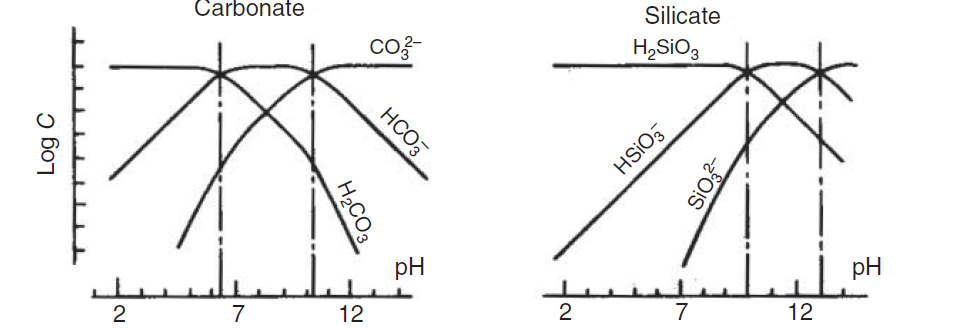
\includegraphics[width=0.7\textwidth]{Billeder/teori/carbonate_silicate.png}
    \caption{pH pC Carbonate + Silicate}
    \label{fig:pH_pC}
\end{figure}

kilde = \citep{WaterChemistry1980}